\documentclass[12pt]{report}

% Paper Dimensions
%\textwidth = 5.5 in \textheight = 8.5 in \oddsidemargin = 0.5 in
%\evensidemargin = 0.5 in \topmargin = .5 in \headheight = 0.0 in
%\headsep = 0.0 in \footskip = .5in
%\parskip = 0.3mm
\parindent = 0.5in
\linespread{1.6} %gives the line spacing.  the higher the number the larger the spacing.
\usepackage{geometry}
\geometry{
    left = 1.5in,
    right = 1.0in,
    top = 1.0in,
    bottom = 1.0in,
}

% Symbols
\usepackage{amsmath,amssymb,url,bm}
% Formatting
\usepackage{multicol, csquotes, scrextend, color, titlesec}
%% Tables, Figures
\usepackage{longtable, booktabs, pdflscape, placeins}
%% Chapter header formatting
\usepackage[T1]{fontenc}
\definecolor{gray75}{gray}{0.75}
\newcommand{\hsp}{\hspace{20pt}}
\titleformat{\chapter}[hang]{\Huge\bfseries}{\thechapter\hsp\textcolor{gray75}{|}\hsp}{0pt}{\Huge\bfseries}
% Images
\usepackage{graphicx, float, caption, subcaption}
% Indexing
\usepackage{bookmark}
%Bibliography stuff
\usepackage[nottoc,numbib]{tocbibind}
\usepackage{datetime}

\begin{document}
%------------------- TRACK DRAFT CHANGES ---------------------------
% Date
\chapter*{Draft Date: \\ \today \\ \currenttime}
\newpage

%------------------- ABSTRACT ---------------------------------
\chapter{Abstract}

%------------------- INTRODUCTION ---------------------------------
\chapter{Introduction}
\section{Background}
% Trends/stats
Homelessness in the United States persists in spite of various efforts to assist the many people experiencing it. The United States has seen a decrease of 42\% in homelessness since the Department of Housing and Urban Development (HUD) began tracking it in a nationally coordinated manner in 2005; however, HUD recorded over 442,000 people experiencing homelessness in 2020 through their Point in Time Count program \cite{PITcount}. 

This study focuses on homelessnes in Spokane County, Washington. Washington State has seen a decrease in homelessness of 28\% from 2005 to 2020, but according to HUD still retains over 17,000 people experiencing homelessness. In Spokane County homelessness has decreased by 32\% since 2005 and 1,244 people were recorded as experiencing homelessness in 2020 \cite{PITcount}. These numbers include individuals sheltered in emergency shelters, sheltered in transitional housing, and unsheltered \cite{PITcount}.

\begin{figure}[H]
    \begin{minipage}{0.5\textwidth}
        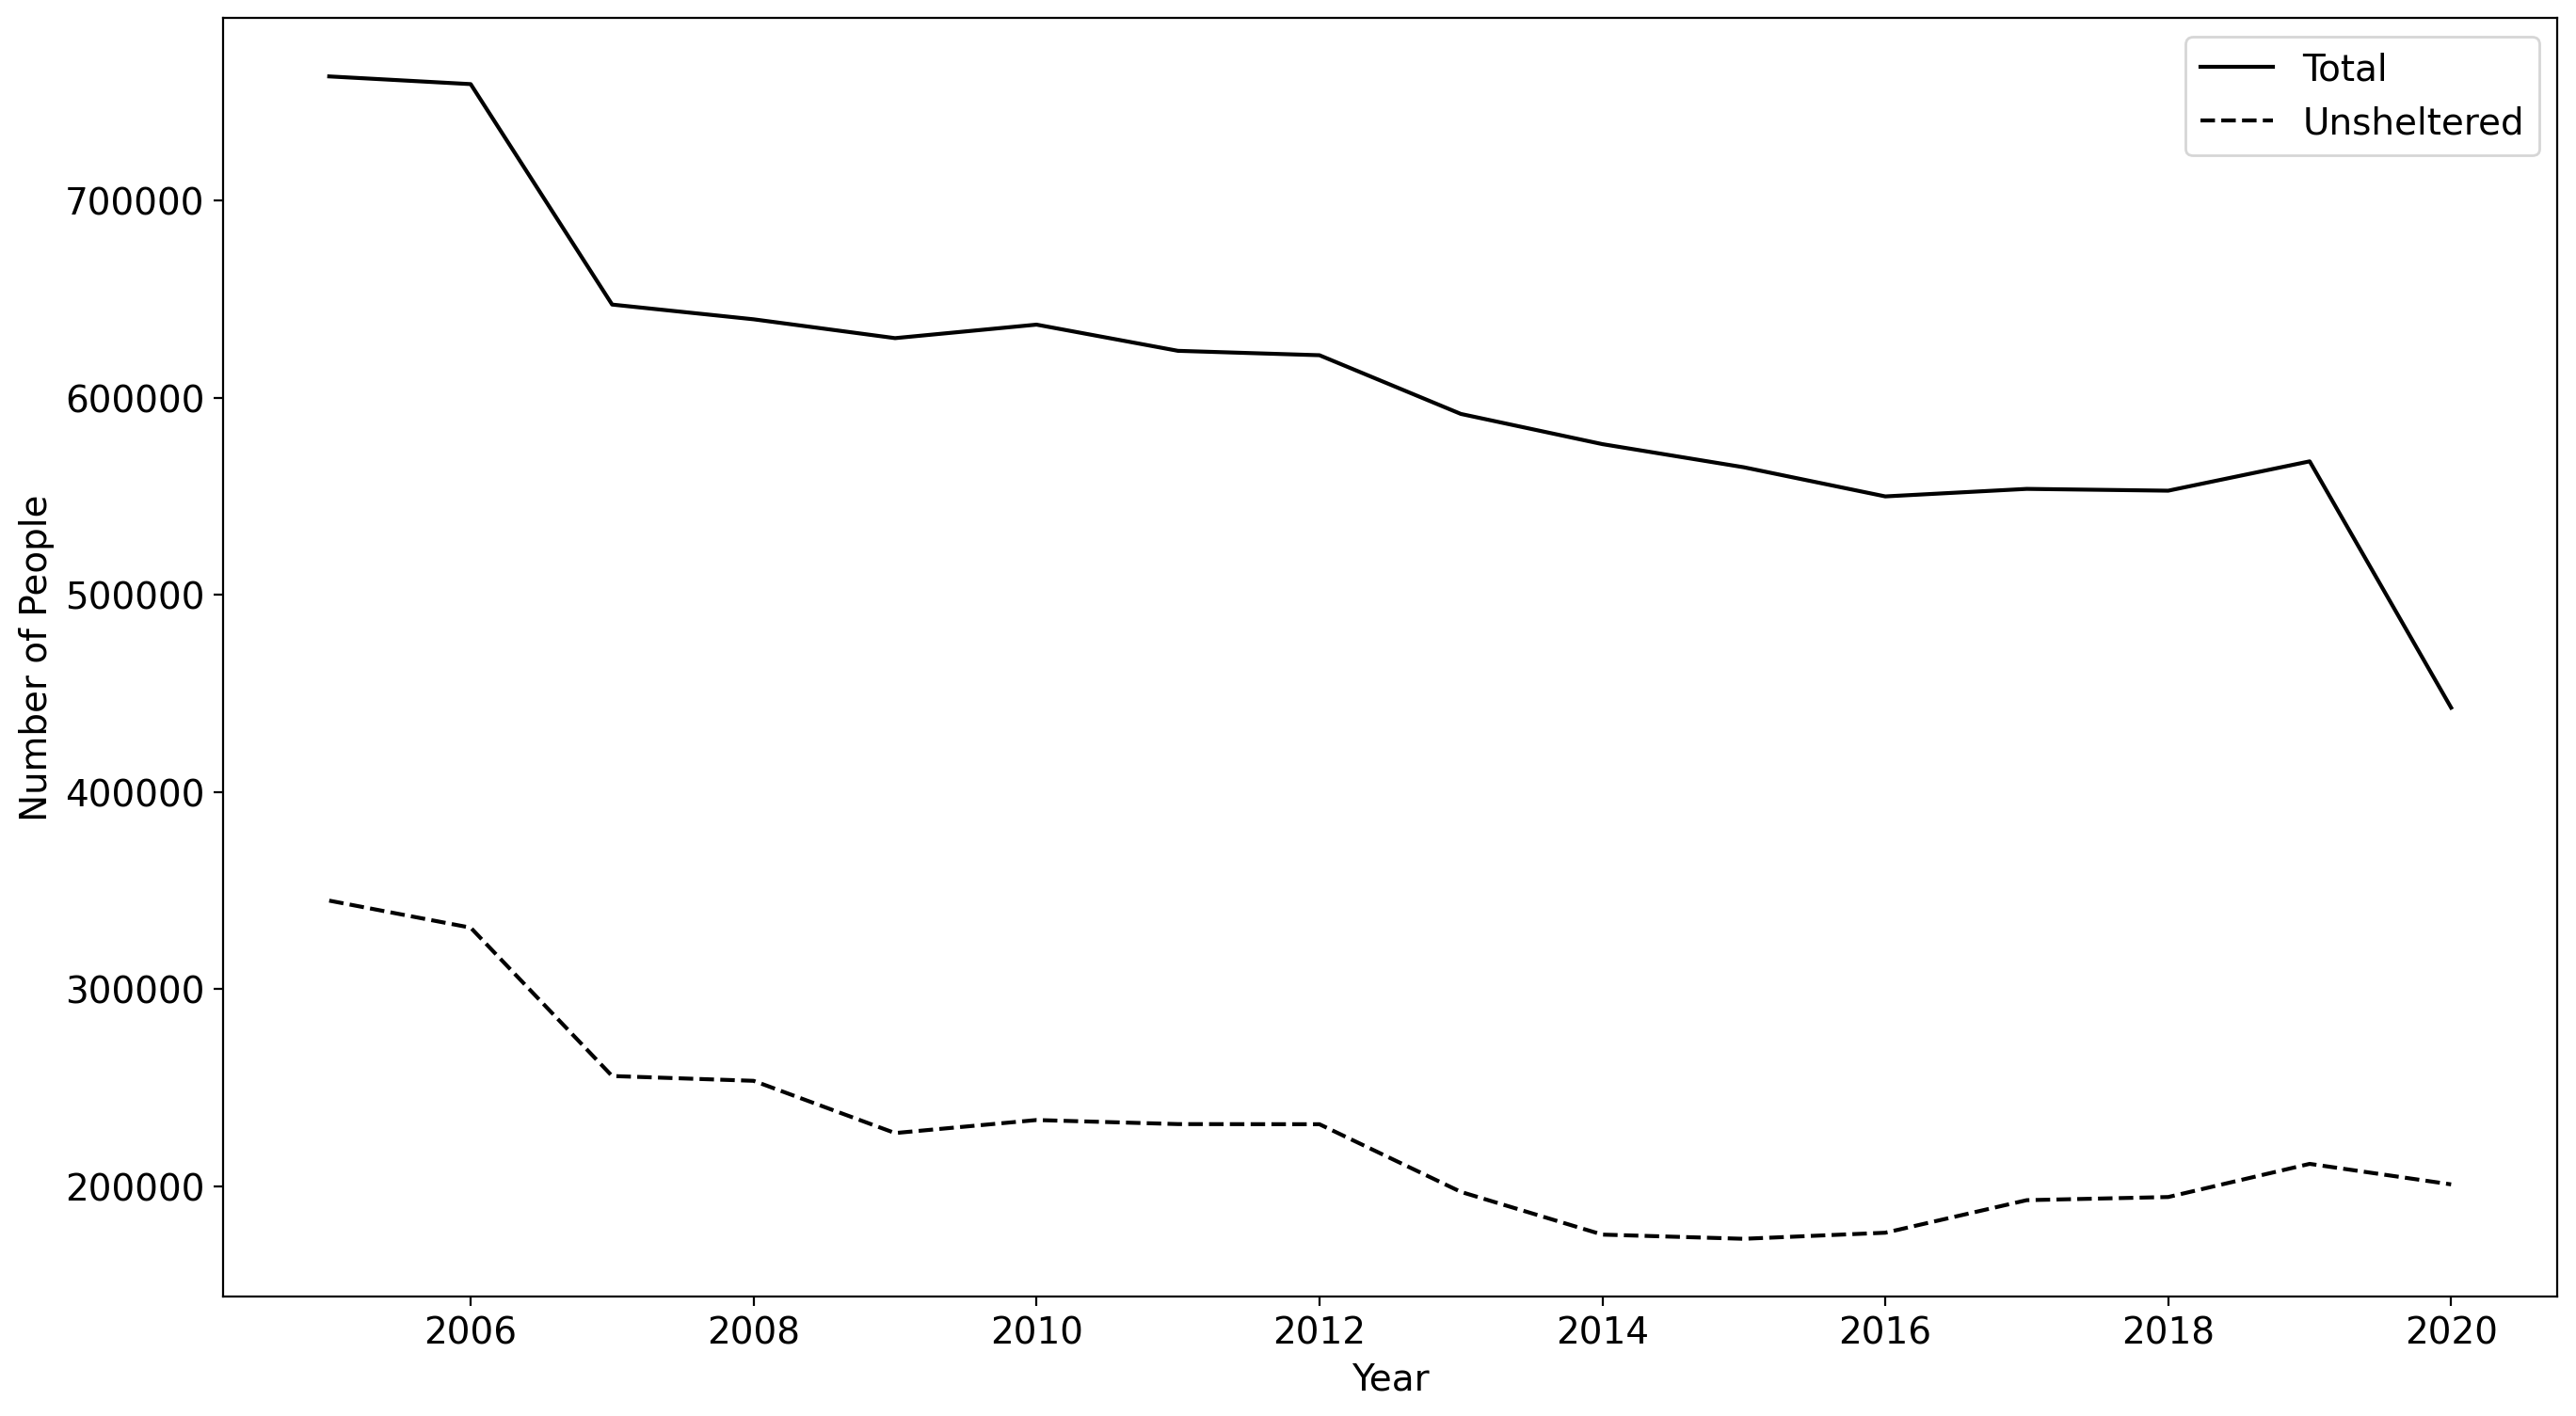
\includegraphics[width=\textwidth]{../img/homelessness_usa.png} 
    \end{minipage}
    \begin{minipage}{0.5\textwidth}
        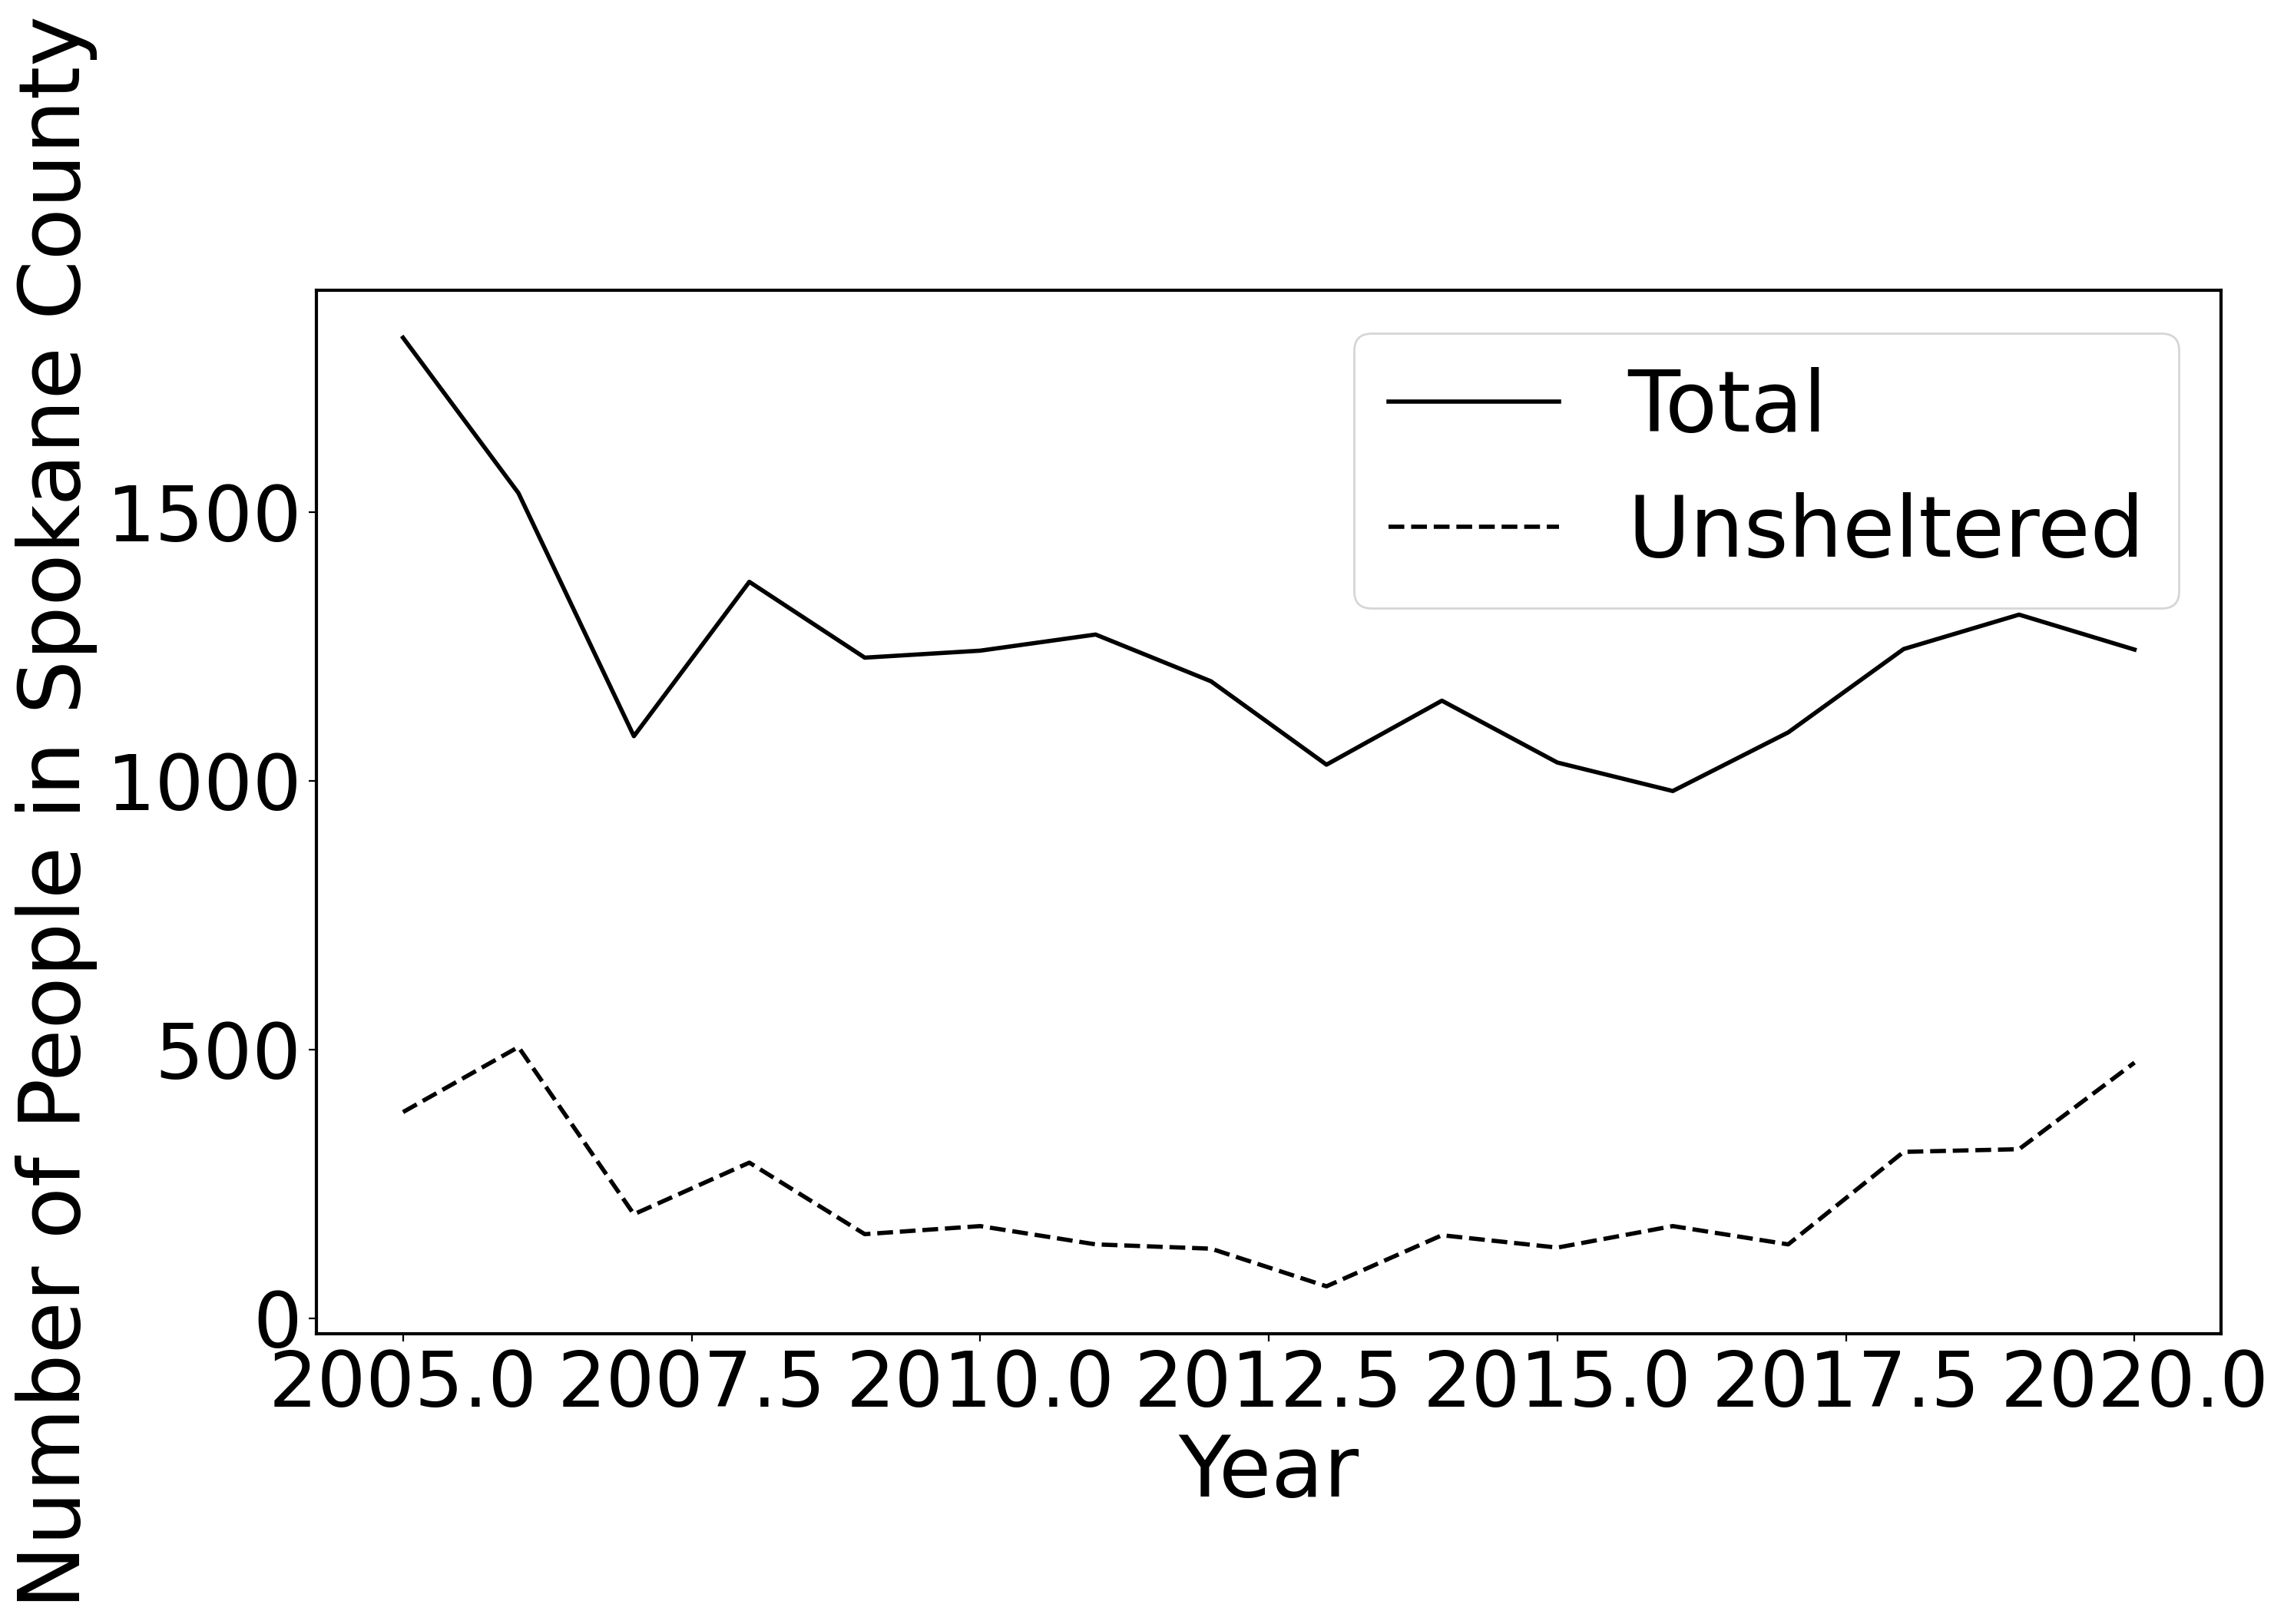
\includegraphics[width=\textwidth]{../img/homelessness_spokane.png}
    \end{minipage}
    \caption[Annual Homelessness in US and Spokane County]{Annual Homelessness in US and Spokane County.
    \cite{PITcount}}
    \label{fig:Homeless_US_Spokane}
\end{figure}

% Definition of Homelessness
For this study we use the definition of homelessness used by the agencies that collected the homelessness data. They use the ``Category 1: Literally Homeless'' definition presented by HUD:
\begin{displayquote}[\cite{hud_hmls_def}]
1) Individual or family who lacks a fixed, regular, and adequate nighttime residence, meaning: \\
(i) Has a primary nighttime residence that is a public or private place not meant for human habitation; \\
(ii) Is living in a publicly or privately operated shelter designated to provide temporary living arrangements (including congregate shelters, transitional housing, and hotels and motels paid for by charitable organizations or by federal, state and local government programs); or \\
(iii) Is exiting an institution where (s)he has resided for 90 days or less and who resided in an emergency shelter or place not meant for human habitation immediately before entering that institution
\end{displayquote}

% Efforts to combat homelessness
Programs focused on providing assistance to people experiencing homelessness are having an impact. HUD's January 2019 survey found that ``there were 144,000 more permanent supportive housing (PSH) beds dedicated to people with chronic patterns of homelessness than there were in 2007 (a 380\% increase)'' \cite{2019AHAR}. Likely because of this increase in resources the rate of chronic homelessness (people who have experienced homelessness for at least 12 months in the last three years) has declined by 20\% from 2007 to 2019 \cite{2019AHAR}. Current assistance programs and the positive impacts they have on people in need represent a significant accomplishment, but these programs largely focus on providing support to people already experiencing homelessness. This type of assistance program can only help so much. In order to substantially reduce and eventually end homelessness altogether, homelessness prevention programs must be utilized. 

We will refer to programs as homelessness prevention programs (HPPs) if they focus on preventing people from experiencing homelessness. These programs include permanent deep rental housing subsidies, eviction prevention programs, community based services such as short term financial assistance, education, and job placement. Homeless assistance programs (HAPs), we shall say are those that are specifically aimed at people who are currently experiencing an episode of homelessness and include shelters and other emergency services. There are two aspects of HPPs that make them more attractive than HAPs. The first is cost. The services that HPPs typically offer are less expensive for taxpayers than those provided by HAPs \cite{shinn2019homelessness}. The second reason is that if the HPP is successful it will spare people the trauma typical of experiencing homelessness.

\subsection{Cost Effectiveness of Homeless Prevention Programs}
Research has shown that many HPPs are cost effective in practice, meaning people identified as at-risk and assisted with a HPP cost less than people who experience homelessness and are assisted by a HAP. A study on permanent deep rental housing subsidies, one of the most promising types of prevention programs, found that ``among the 67 percent of families who successfully used their [rent subsidy] voucher to lease housing, homelessness was prevented entirely'' \cite{shinn2019homelessness} (Page 5). Another study analyzed an eviction prevention program from 2010 to 2012 in Chicago that distributed rent assistance based on at-risk individuals calling a Homelessness Prevention Call Center. Researchers found that six months after a person had called in, only 0.5\% of those who received financial aid experienced homelessness, while 2.1\% of those who did not receive aid experienced homelessness. The program was especially helpful for the lowest income callers and the authors claim could have been more efficient with better targeting \cite{evans2016impact}. In New York City a program called HomeBase provides community based services to at-risk individuals. Two papers have concluded that this program is cost effective at preventing homelessness \cite{rolston2013evaluation} \cite{goodman2016homelessness}. 

Homeless prevention is effective on a large scale as well. In 2009 the United States government distributed \$1.5 billion through the Homeless Prevention and Rapid Rehousing Program which promoted HPPs. According to the National Alliance to End Homelessness this spending and promotion of HPPs largely caused the 1\% decline in homelessness between 2009 and 2011, which is notable considering the economic recession during that time \cite{shinn2013efficient}.

\subsection{Halting the Pathology of Homelessness}
There is one important aspect of the pathology of homelessnes that is likely the cause of HPPs' effectiveness - a gradual divergence from financial stability. We hypothesise that individuals that eventually experience homelessness begin thier journey as indistinguishable from the healthy population. As time moves forward, these individuals begin to shows signs of financial distress and become more and more separate from the healthy population (and more identifiable as at-risk) as they progress towards experiencing homelessnes. As this progression occurs, and especially once an individual experiences an episode of homelessness, it becomes more difficult to change their financial trajectory and help them reestablish their independence. This hypothesis is supported by Shinn's ``Efficient Targeting of Homelessness Prevention Services for Families,'' which found that ``[t]he single best predictor of eventual homelessness is having previously been in a shelter'' \cite{shinn2019homelessness} (Page 3). The point of HPPs is to change the trajectories of at-risk individuals early in this process. If an intervention is performed early in the process, only a minor course correction is necessary. 

There does not appear to be any significant portion of the population that is too high-risk for HPPs to assist. In a study on New York's HomeBase program in 2013 it was found that ``No level of risk was too high for families to benefit from services and, indeed, even in the highest decile of measured risk, a majority of families avoided shelter'' \cite{shinn2013efficient} (Page 3). This finding is important because it provides statistical backing to the notion that no one is beyond help. It also informs which part of the population HPPs should focus on - people who are predicted to have the highest risk of experiencing homelessness.

According to a 2019 study by the California Policy Lab, HPPs should be both effective and efficient. An \textit{effective} program prevents people from experiencing homelessness that would have if they had not been provided assistance. An \textit{efficient} program only provides assistance to those who actually need it \cite{PredictPreventHmlsnsLA}. A good analogy here is that HPPs striving to provide assistance to a certain type of person, those who will experience homelessness, is like casting a net to catch a certain type of fish. Programs that ``cast a large net'' by assisting many people can easily be effective because they are likely to prevent a large number of people from experiencing homelessness. However, it is difficult for such a program to be efficient because it will inevitably provide assistance to many people who would not experience homelessness even if they did not receive assistance. In a similar way a program that ``casts a small net,'' targeting the people identified as most at-risk of experiencing homelessness, can be highly efficient by only providing assistance to people who would have experienced homelessness, but is likely less effective because some people who do not receive assistance will still experience homelessness simply because they were not identified as the most at-risk. The ideal situation is a program that assists all the people who would experience homelessness and none who would not. This ideal is almost certainly unattainable in practice due to the difficulty of identifying who will experience homelessness. The key to providing this targeted assistance is correctly identifying the most at-risk individuals and doing so as early as possible in order to give them the best chance at correcting their trajectory.

\section{Homelessness Prediction Background}
Identifying individuals to enroll in HPPs is a difficult task because everyone is a candidate; anyone might experience homelessness at some point in the future. The path to homelessness may be different for different individuals and people may persist in a high-risk-of-homelessness state without ever experiencing an episode of homelessness. Only when a tipping point is reached - one too many bills are due close together, a parking ticket, a medical expense, etc. - does someone lose their housing and experience an episode of homelessness \cite{o2004wrong}. Because of this ability for some individuals to maintain a state of financial distress but never experience homelessness, even the best prediction models will likely produce false positives, that is, predict some people as having a high risk of experiencing homelessness when they never actually do.

Currently, screening for HPPs is almost entirely performed by healthcare workers. Using surveys, their experience, and their intuition they evaluate each individual and determine who gets which aid and how much. There are at times high volumes of individuals seeking assistance, especially in large cities, which slows down this system. Another issue is that the evaluators have biases which may affect their decisions about who gets aid and who does not \cite{shinn2019homelessness}.

The use of statistical models as a screening method shows promise in this area. Statistical models add more objectivity to the screening process; any bias they contain can be measured and corrected. One study found that the use of a screening model reduced the number of applicants to HPPs who were turned down and then eventually entered a shelter from 28.4\% to 8.1\% \cite{shinn2019homelessness}. Screening systems using statistical models are also fast and easily automated which reduces the burden on healthcare workers, are less expensive to operate, and can help speed up the overall process of providing assistance to those in need.

\section{Homelessness Prediction in the Literature}
The topic of identifying individuals at risk of homelessness is minimally studied in academia. There are several reasons for this with the first being that before 2009 there were very few HPPs in the United States to study. This was largely due to political unpopularity and the difficulty in evaluating HPPs \cite{colburn2014federal}. The effectiveness of HPPs is the number of people prevented from experiencing homelessness, but who would have experienced homelessness if unassisted and who would have self corrected? Prior to 2009 and still the majority of programs related to homelessness today are HAPs. 

Another reason research on this topic is limited is the difficulty in collecting relevant data. A study by the California Policy Lab in 2019 found that the top predictors for homelessness were from most important to least: having previously experienced homelessness, prior receipt of social safety net benefits, interactions with any of: the Department of Human Services, the Department of Mental Health, the Sheriff's Department, or Probation, with a greater number of interactions with shorter time intervals also indicating greater risk. Other indicators were found to be visiting multiple service locations and residing in certain geographical areas \cite{PredictPreventHmlsnsLA}. The challenge is that these data are fragmented across government and sometimes private agencies with little history of coordination or standard data keeping practices between them.

Nearly all the relevant data to homelessness is highly personal in nature so access is restricted. The system our project used for data acquisition is to have a central agency that is given all data from the relevant agencies through secure channels. This central agency matches and combines the data from the different sources, then de-identifies it. This process entails creating a map of agency-generated identifiers for each sensitive aspect of the data, then replace all the original values with these new identifiers. For example, each address is replaced by a unique address identification number so that the agencies working with the data cannot identify to who or where the data corresponds. This data handling structure is practiced and recommended by Los Angeles County’s Enterprise Linkages Project, which handles similarly sensitive data \cite{byrne2012angeles}.

\section{The Potential of Utility Customer Data}
Our project uses utility customer payment data to predict risk of experiencing homelessness. This data source is attractive for two key reasons. First, it contains information related to individuals' financial health such as utility bill amounts, amount owed to the utility company, and number of times a bill payment was missed. Risk of homelessness is closely linked with an individual's financial health.

The second reason why utility data is attractive is its ubiquity. Almost all households pay some form of utility bill, so this data is available for nearly everyone across the U.S. It may exist in different forms and in different agencies, but similar information on amounts owed and payment default likely exists in all utility-customer situations. If it were a source of useful information in predicting homelessness, any derived models could be used anywhere in the U.S. using similar data sources. 

\section{Intended Use of Prediction Model}
The product of this project, the model, is intended for use by an HPP to identify the target population of people most at-risk of experiencing homelessness. A convenient output format is a ranked list of individuals and their associated risks of experiencing homelessness. With this information, the HPP can assist at-risk individuals in two convenient ways:

\begin{itemize}
    \item Option 1
    \begin{enumerate}
        \item Assess the pool of resources available to assist at-risk individuals,
        \item determine the number of people that can receive aid based on this pool, say $n$,
        \item and simply choose the $n$ individuals with highest predicted risk.
    \end{enumerate}
    \item Option 2
    \begin{enumerate}
        \item Analyze the list of individuals and their risks of experiencing homelessness,
        \item choose a threshold risk value,
        \item then assist all individuals above that threshold. This method may be appropriate if there is a large gap in predicted risks.
    \end{enumerate}
\end{itemize}

%------------------- Materials and Methods ---------------------------------
\chapter{Materials and Methods}
\section{The Data}
The data used for this project was obtained from Avista Utilities and the City of Spokane. Avista Utilities provided monthly residential customer billing information for electricity and natural gas utilities. The City of Spokanen provided monthly combined water, sewer, and garbage billing information as well as outcome data on who has been recorded as experiencing homelessness and at what times.

% Limitations of Data
The data used for this project is inherently limited in its scope to some degree. Though the main benefit of using utility data is to capture as much of the population as possible, still only people who have been involved with a utility billing account are captured. The data captures 84,345 people, about 16\% of the total Spokane County population which was 522,798 in 2019 \cite{SpokanePop}.

Another major limitation of the data is incomplete outcome measurement. Positive outcomes (if someone experiences homelessness) were gathered from the City of Spokane's Community Management Information System (CMIS), an organization that collects data from various HAPs in the Spokane area. Everyone who did not appear in the CMIS database was assumed to be a negative case (did not experience homelessness). Positive cases are gathered by this method with a high degree of confidence, but some people who experience homelessness may be mis-labeled as negative cases. This could occur if a person moved out of the CMIS's data collection area before experiencing homelessness or if they simply never sought assistance.

% Matching + De-Identifying
Initial data matching and de-identifying was performed by the data team at Avista Utilities. This process involved gathering the data from its sources and matching on name, address, and month. After matching, the data was de-identified by replacing any identifiable characteristics of the data such as name and address with internally generated identification numbers. Additional matching was performed by the authors. After this process, the data contained information on 85,345 people who have been listed as the main account holder on a utility billing account in Spokane County from December, 2015 to December, 2020. For each person there are monthly entries with information about thier utility billing activities. 

\subsection{Association Metrics}
To measure relationships between variables in the data, different association metrics were used depending on the variable types. The following is a list of variable pairing types and the metric used to measure strength of association between the variables: absolute value of Spearman Correlation for continuous-continuous, Point-Biserial Correlation for binary-continuous, Theil Uncertainty Coefficient for categorical-categorical, and Correlation Ratio for continuous-categorical(with more than two levels).

\subsection{Data Homogeneity}
% Data Homogeneity - add this to discussion?
When attempting to learn patterns and relationships from data, it is important to understand if certain parts of the data are different from other parts. For this project we are distinguishing between positive and negative cases, but there are many other ways the data can be divided. One important division is by the year in which the data was collected, from 2015 to 2020. Perhaps there were different relationships between the tracked variables and homelessness during different years. 

The year 2020 was expected to contain different relationships than the previous years because the COVID-19 pandemic caused people and the utility agencies to behave differently than they had in previous years. For example, for the greater part of 2020, the utility agencies tracked in our dataset did not perform service shut-offs as they had in previous years \cite{white2020utilities}. 

To investigate if there was a difference in the associations between the variables and the outcome in different years, the data was split by year, the strength of association of each variable with the outcome was measured, these strengths were then ranked, and the rankings were compared from year to year. Figure \ref{fig:corrRankByYear} shows a plot of these ranks. Surprisingly, they appear to be very similar from year to year. A numerical approach was also taken by computing between years the Spearman's Rank Correlation for the association strengths of variables to outcome measure. These are displayed in the association heatmap in Figure \ref{fig:corr_years}. All the association values are 0.895 or larger, indicating that the rankings of the associations of explanatory variables to the outcome within each year are very similar between years. This means that the important relationships within the data are similar from year to year, so all available years, 2015 to 2020, were included in further analysis and modeling as a single group. Note that years 2020 and 2016 are the most different. This is expected because they are far apart in time. Interestingly, 2020 and 2015 are very similar.

\begin{figure}[h]
    \centering
    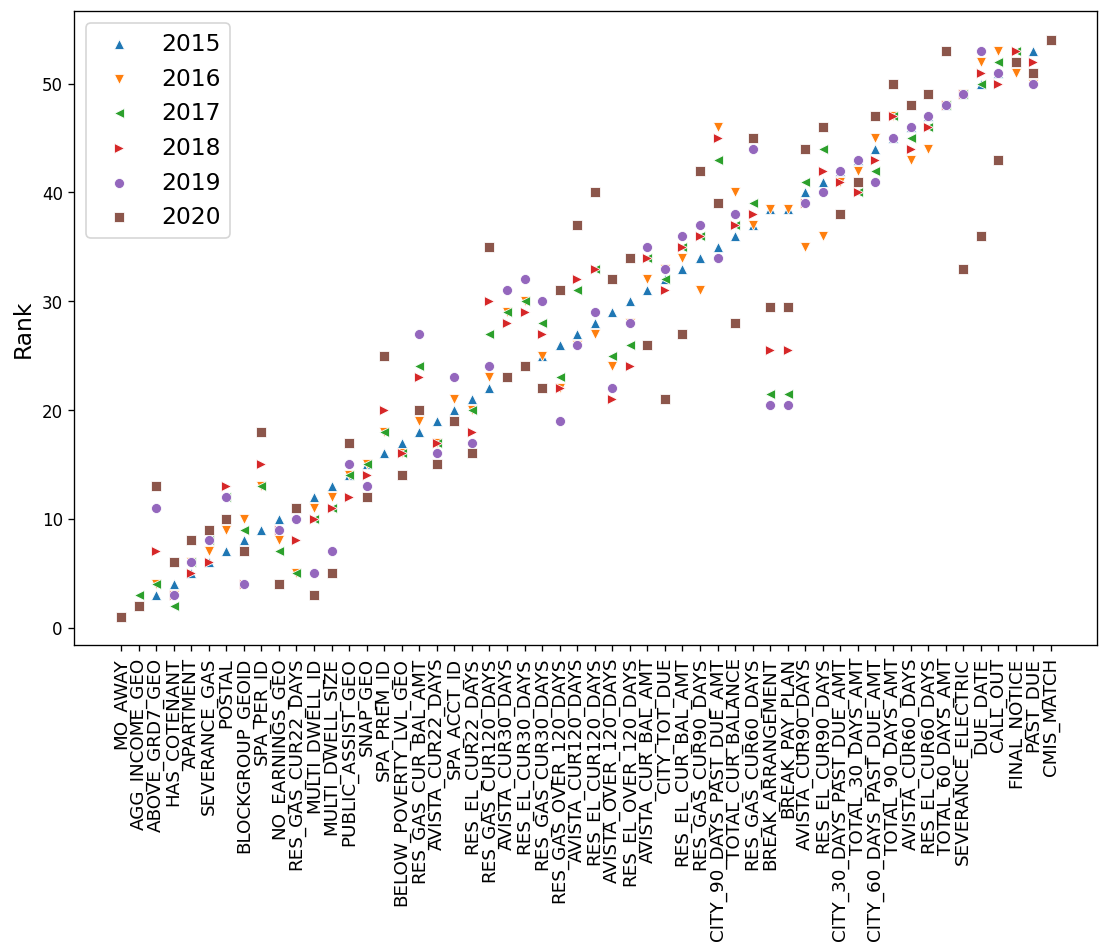
\includegraphics[width=\textwidth]{../img/corrRankByYear.png}
    \caption[Ranks of variable correlation by year]{The ranks, by year, of the strengths of association between each explanatory variable and the outcome of homelessness (CMIS\_MATCH). Values sorted by the 2015 ranks.}
    \label{fig:corrRankByYear}
\end{figure}

\begin{figure}[h]
    \centering
    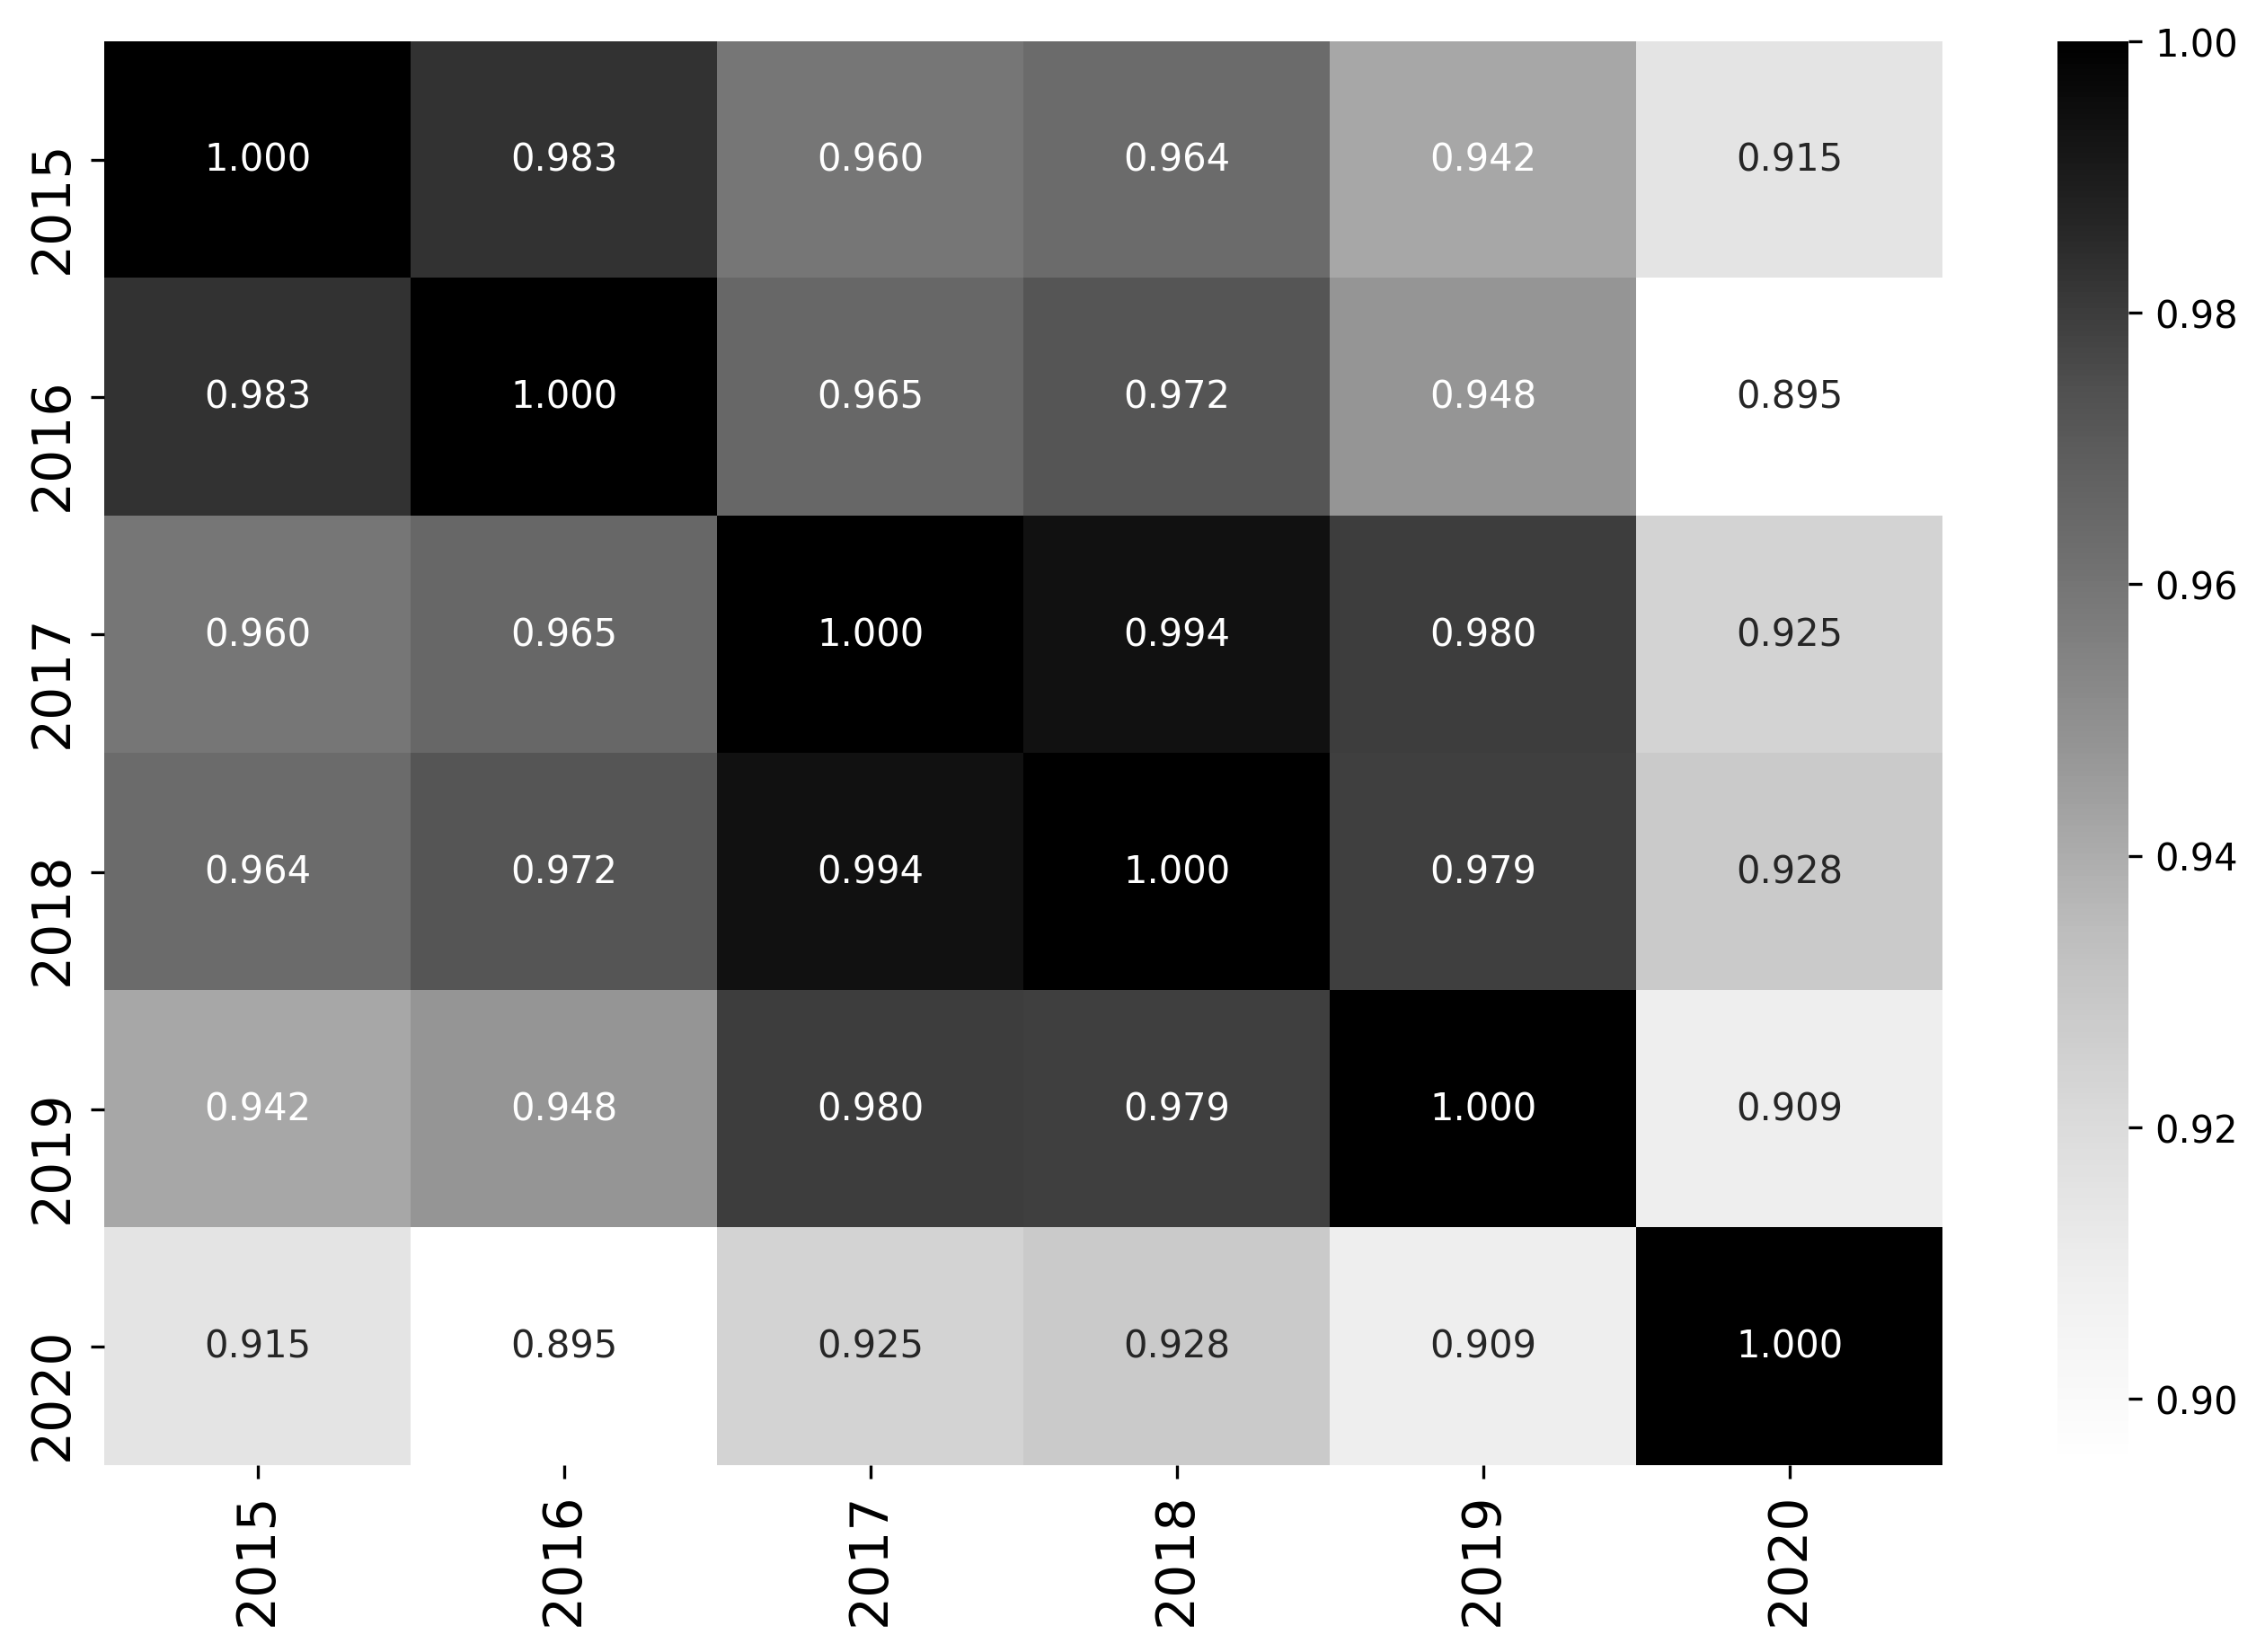
\includegraphics[width=0.7\textwidth]{../img/corr_years.png}
    \caption[Correlation of variable correlation order by year]{The associations, measured with Spearman's Rank Correlation, between the rankings of strengths of association between explanatory variables and the outcome of homelessness (CMIS\_MATCH). All are at least 0.895, indicating strong association and that the associations over the years are similar to each other.}
    \label{fig:corr_years}
\end{figure}

% Characteristics Over Time
Time is hypothesized to be an important factor in the pattern of how the risk of homelessness is indicated in individuals. Specifically, as an individual gets closer to the time when they experience homelessness, they likely exhibit characteristics that are more distinct from the rest of the population and, as a result, should be easier to identify. 

The relationships between one of the key variables and time was investigated in a series of Figure \ref{fig:PN_mo_away_on_TOTAL_60_DAYS_AMT}. This figure shows how the amount owed by an individual in all utility bills changes as individuals get closer to the time they experience homelessness. The horizontal axis is number of months until homelessness, so 0 is the last month we have utility billing data on the individual before they experience homelessness. The solid line with shaded error margin shows the mean and mean +/- 1 standard deviation for all positive cases during each MO\_AWAY in that variable. The mean and mean +/- 1 standard deviation for negative cases is also plotted for comparison, the dashed-dotted line and dashed lines, respectively, but these do not change over time since negative cases have no meaningful value for the MO\_AWAY outcome measure.

\begin{figure}[h]
    \centering
    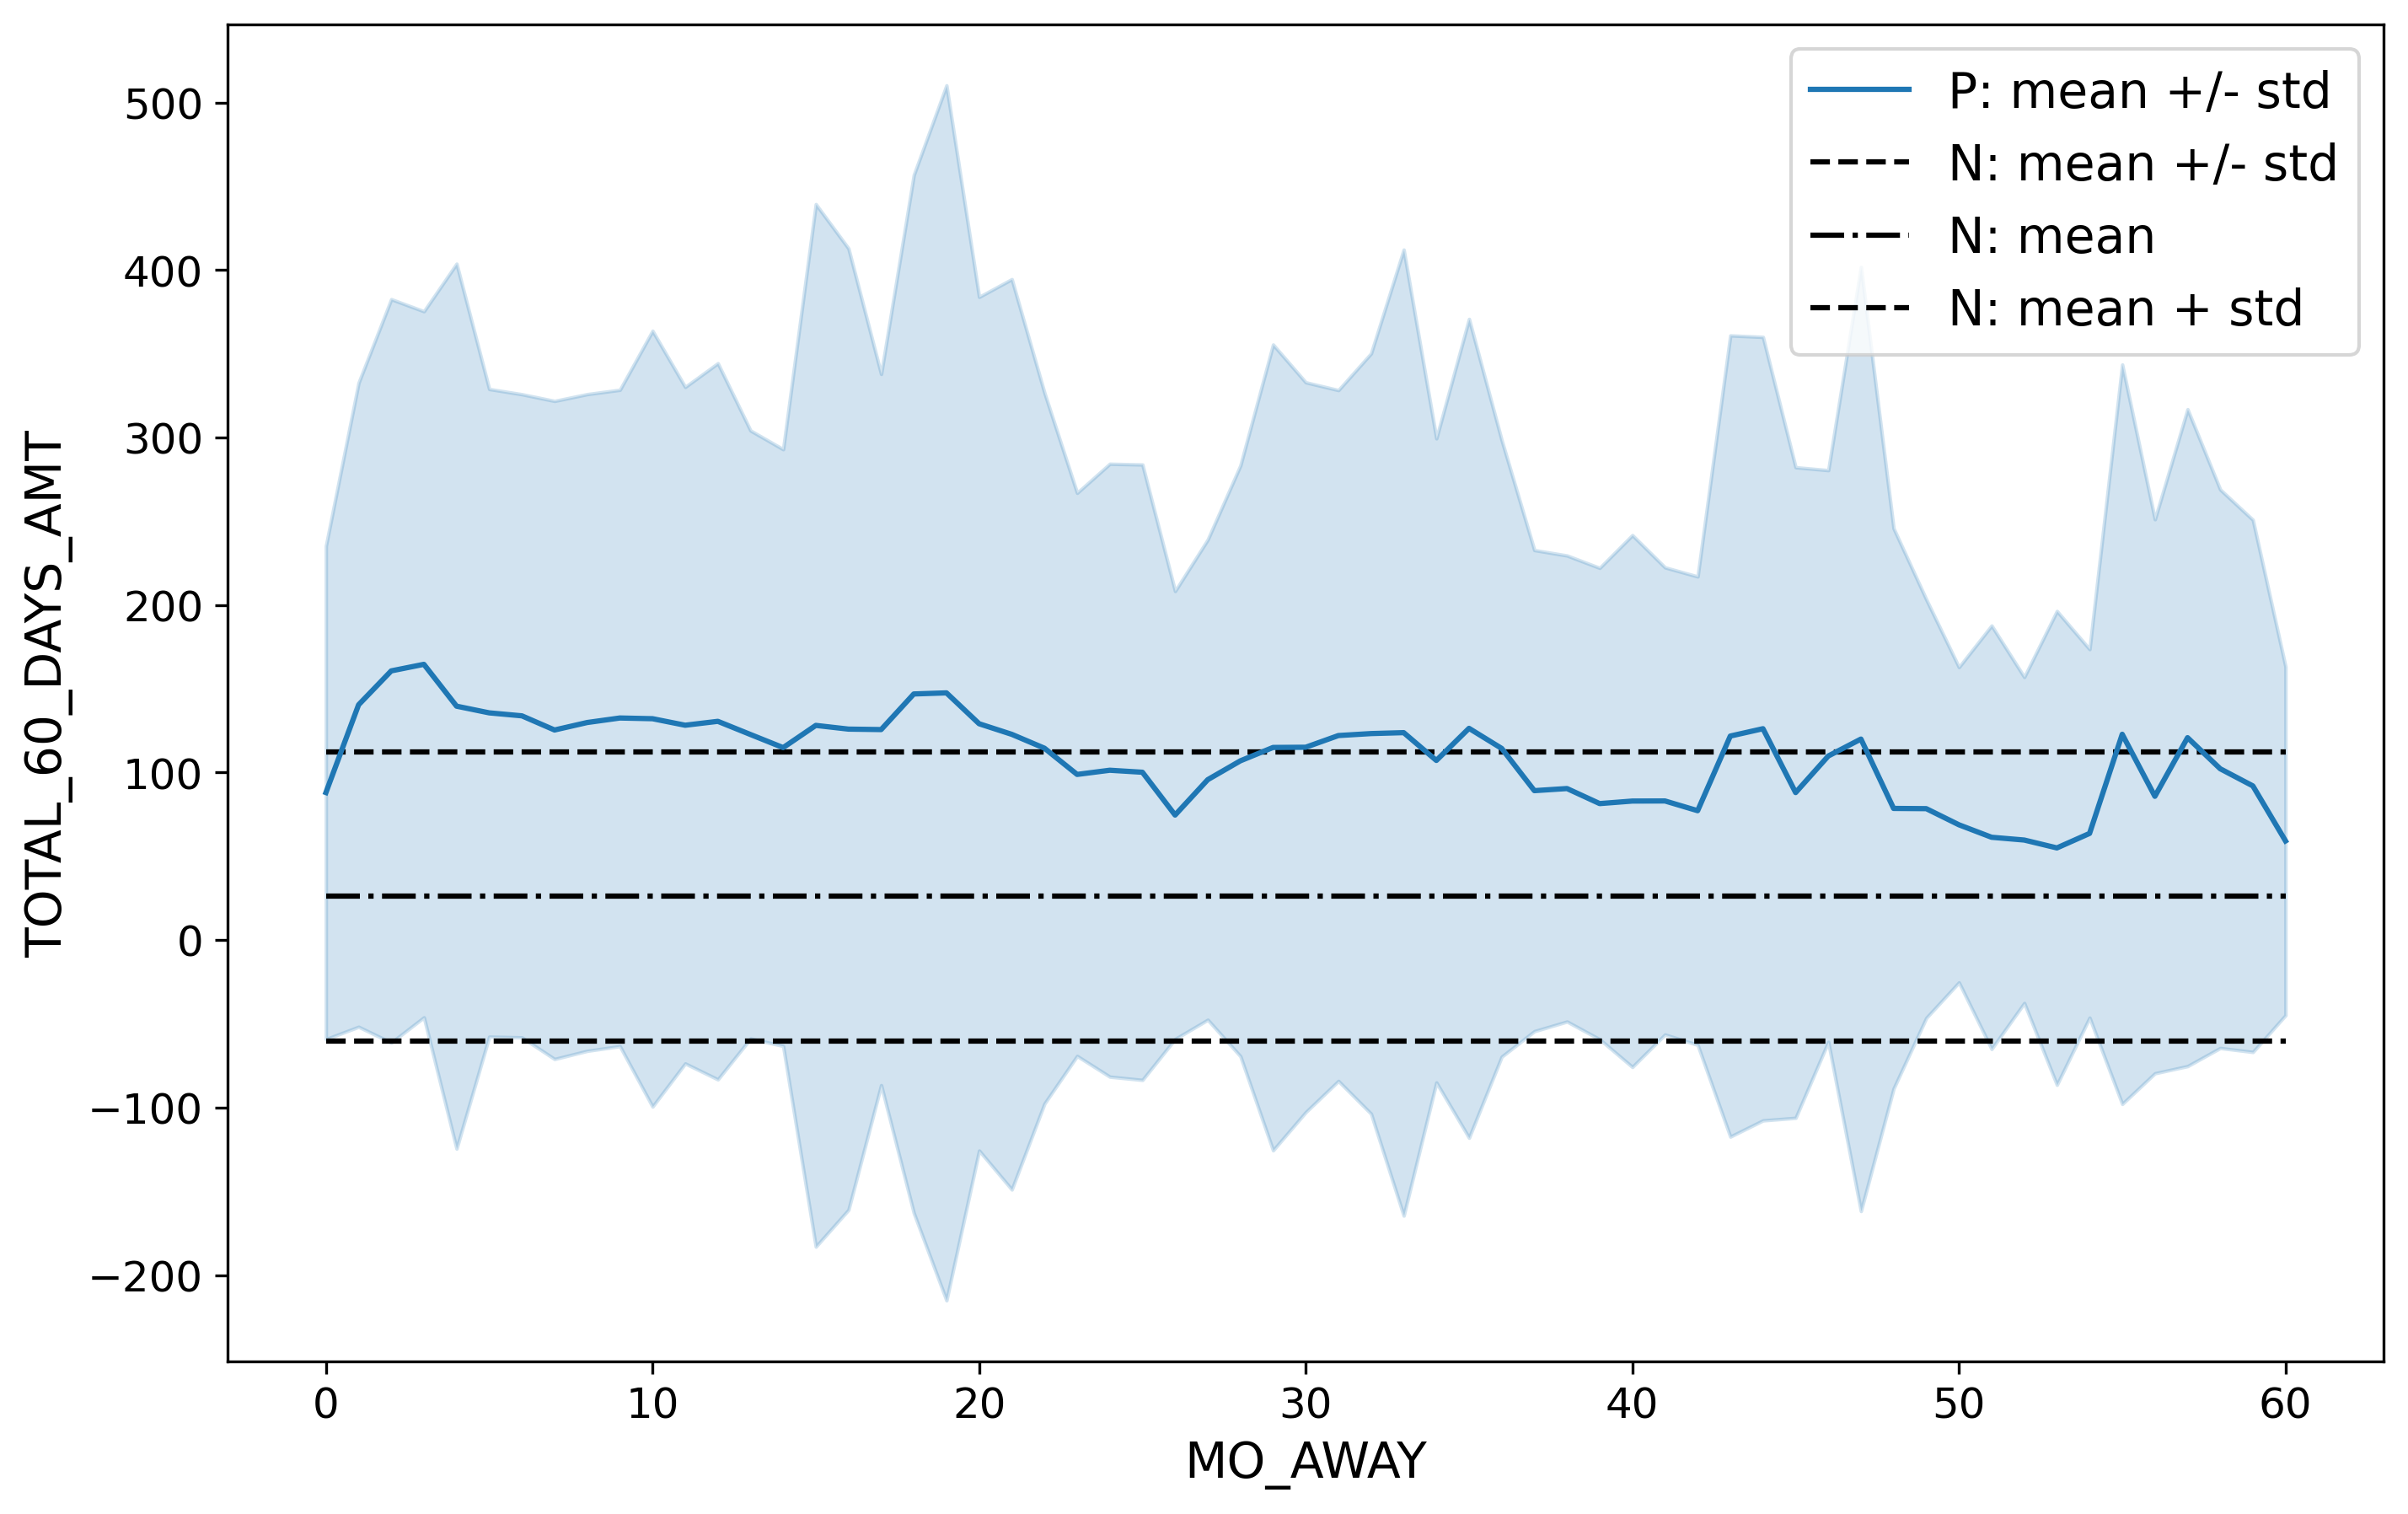
\includegraphics[width=\textwidth]{../img/PN_mo_away_on_TOTAL_60_DAYS_AMT.png}
    \caption{Positive and negative cases on TOTAL\_60\_DAYS\_AMT over time.}
    \label{fig:PN_mo_away_on_TOTAL_60_DAYS_AMT}
\end{figure}

There is a weak upward trend in TOTAL\_60\_DAYS\_AMT as people get closer to experiencing homelessness in time (towards the left). There is a surprising drop just before individuals experience homelessness. Overall a significant proportion of the positive cases overlap with the negative mean +/- 1 standard deviation. This makes it difficult to distinguish between positive and negative cases using this variable. Other variables show similar trends and even less separation between positive and negative cases; TOTAL\_60\_DAYS\_AMT is the variable most strongly correlated with the outcome of homelessness.

% Data Imbalance
The high degree of imbalance in the dataset, that is, the large number of negative cases, people who were never recorded as experiencing homelessness within the dataset, compared to the small number of positive cases, people who were recorded as experiencing homelessness, was a major challenge to model fitting. Specifically, there were 302 positive cases and 84,066 negative cases. This imbalance adds difficulty to the model's task of distinguishing between positive and negative cases because it is difficult to identify the few positive cases among the many negative cases, especially if there are many negative cases that are similar to the positive cases. In this study identifying the positive cases in the dataset is much more important than the negative cases.

\section{Feature Engineering and Selection}
An effort was made to extract additional information from the data by engineering additional features before it was used to fit models. The amount owed by each person at the start of each month was initially provided as separate attributes: amount owed to Avista in electricity bills, amount owed to Avista in gas bills, and amount owed to the City of Spokane in the combined bill amounts for water, sewer, and garbage. To avoid multicollinearity and concentrate information, the amounts owed were aggregated into a single attribute representing total utility amounts owed. This combined amount was more strongly correlated with the outcome of homelessness than any of the individual amounts owed.

The cumulative number of utility account holders who have lived at each location over time was calculated. This variable relates to the number of people who have moved away from each location and is likely an indicator of a mismatch between the tenant's desire and ability to live at that location. The housing may be desirable to the tenant, but they are forced to move because they cannot afford to stay either because their financial situation has deteriorated or the rent has increased. The housing may also be undesirable to the tenant and their stay was intended to be temporary from the start, in which case moving away would indicate an improvement in financial health. People also move for other reasons besides the housing desirability and their ability to pay rent, but this variable was intended to capture some of the information related to housing desirability and financial health.

The cumulative number of places an individual has stayed was also calculated, but was found to be unhelpful in predicting homelessness. This is an interesting finding in itself and seems to indicate that people who do not experience homelessness move about the same amount as those who do experience homelessness - there was no significant difference between positive and negative cases on this attribute.

% Choosing a response variable
Though the eventual choice of outcome measure is the binary variable of if a person was ever recorded as experiencing homelessness, several others were investigated. One was a numerical variable describing the number of months until an episode of homelessness was analyzed. This posed the challenge of assinging some value(s) to people who were never recorded as experiencing homelessness. The other notable outcome investigated was the binary variable recording if an individual was within six months of experiencing an episode of homelessness. The outcome was chosen to be the variable that had the highest association with the predictor variables based on appropriate association metrics. The following association metrics were used for each type of variable pairing: Theil's Uncertainty for categorical-categorical, Spearman Correlation for numerical-numerical, Correlation Ratio for numerical-categorical with categorical having three or more levels, and Point-Biserial Correlation for binary-numerical.

The choice of outcome measure was based on which was most associated with the available data. Each outcome measure provides different information about the process of experiencing homelessness and each could be used in the modelling stage to answer different questions, but only one was used for this study. Figure \ref{fig:cat_theil} shows the Theil's U values for all categorical variables, including the binary outcome measures.

\begin{figure}[h]
    \centering
    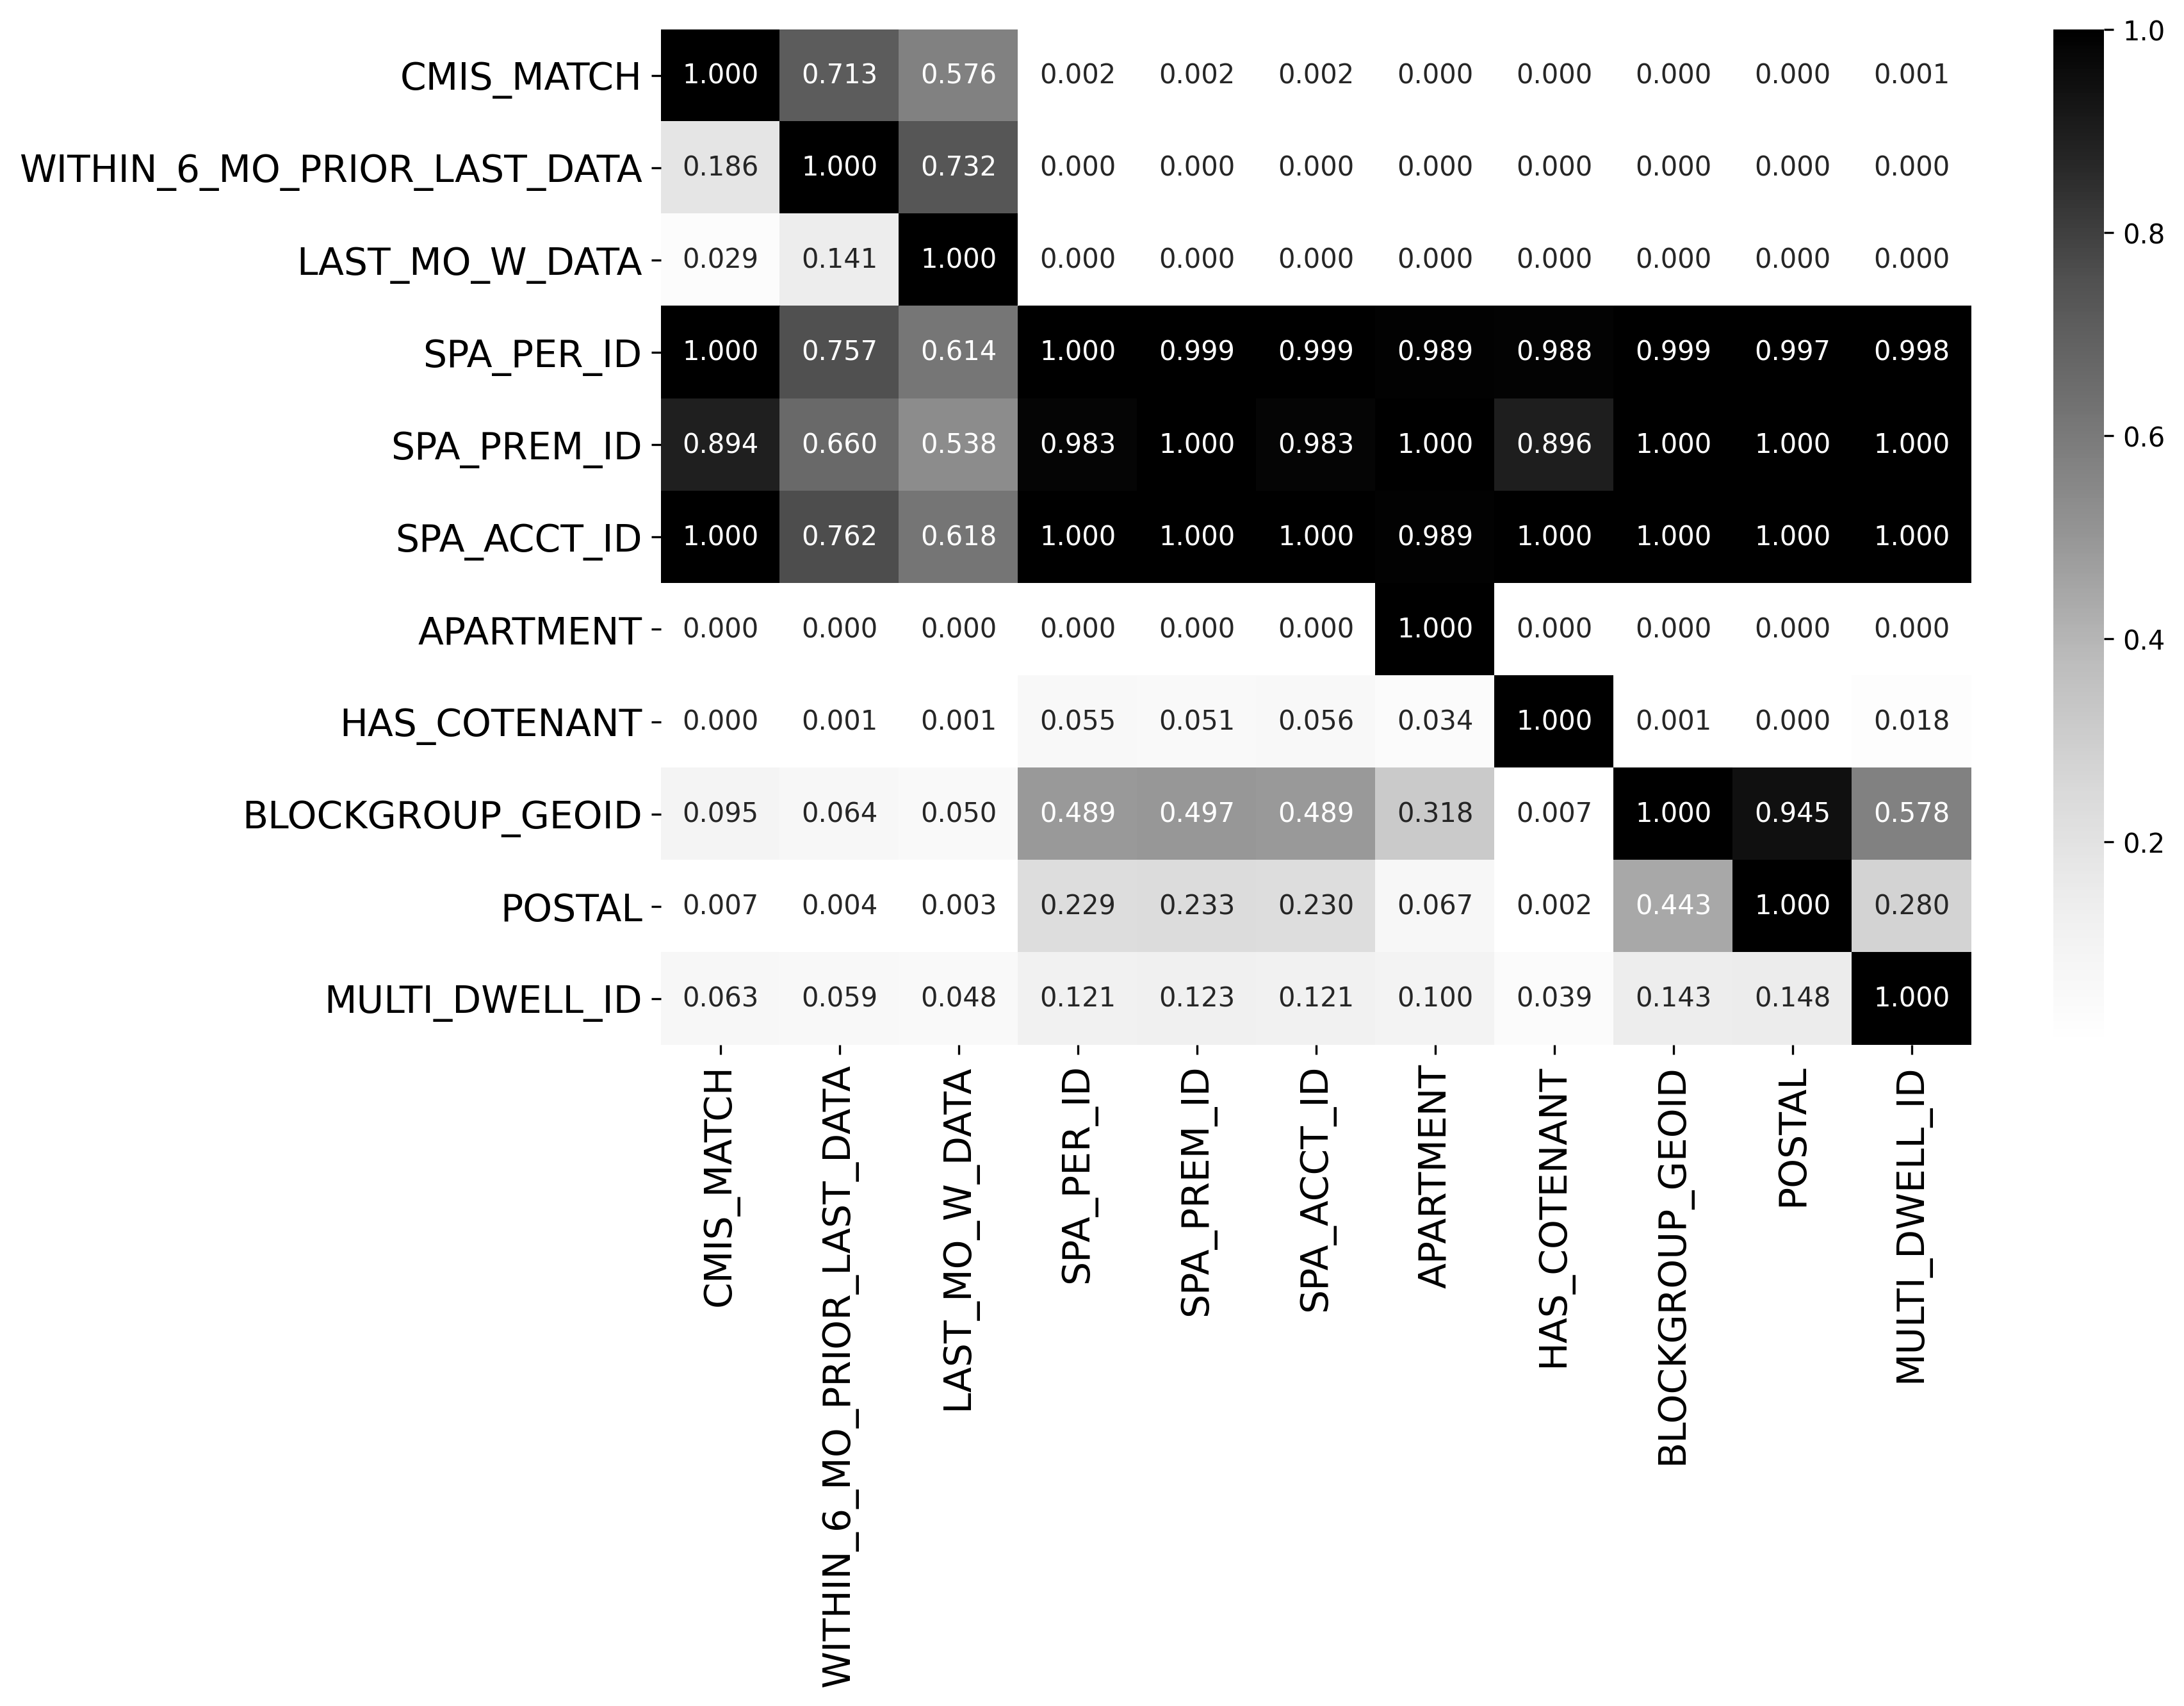
\includegraphics[width=\textwidth]{../img/cat_theil.png}
    \caption[Categorical variable associations]{Theil's U values for all variables considered categorical. Each value corresponds to a $U(X|Y)$ where the $Y$ is on the vertical axis and $X$ is on the horizontal.}
    \label{fig:cat_theil}
\end{figure}

Notice that if a person is uniquely specified by their SPA\_PER\_ID, then most of the other variables are also known, however, if say the POSTAL (postal code) of a data entry is known, then very little can be said about the other variables (except BLOCKGROUP\_GEOID is known to some degree - both are geographical demarcations). CMIS\_MATCH is the best choice of outcome measure because if BLOCKGROUP\_GEOID, POSTAL, or MULTI\_DWELL\_ID are known, there is a better chance of identifying the correct CMIS\_MATCH than the other potential outcome measures. The first fifteen entries with limited decimal resolution are listed here in Table \ref{tbl:assocWithOutcome15}.

\begin{table}[H]
    \centering
    \begin{tabular}{lcccc}
    \toprule
    {} &  MO\_AWAY &  CMIS &  LAST\_MO &  6\_MO \\
    \midrule
    CMIS\_MATCH         &      NaN &        1.00 &             NaN &                          NaN \\
    SPA\_ACCT\_ID        &     0.98 &        1.00 &            0.62 &                         0.76 \\
    SPA\_PER\_ID         &     0.97 &        1.00 &            0.61 &                         0.76 \\
    SPA\_PREM\_ID        &     0.83 &        0.89 &            0.54 &                         0.66 \\
    BLOCKGROUP\_GEOID   &     0.06 &        0.09 &            0.05 &                         0.06 \\
    PAST\_DUE           &     0.06 &        0.07 &            0.01 &                         0.02 \\
    FINAL\_NOTICE       &     0.06 &        0.06 &            0.01 &                         0.02 \\
    MULTI\_DWELL\_ID     &     0.13 &        0.06 &            0.05 &                         0.06 \\
    CALL\_OUT           &     0.06 &        0.06 &            0.01 &                         0.02 \\
    DUE\_DATE           &     0.06 &        0.06 &            0.01 &                         0.03 \\
    TOTAL\_60\_DAYS\_AMT  &     0.05 &        0.06 &            0.01 &                         0.03 \\
    SEVERANCE\_ELECTRIC &     0.06 &        0.06 &            0.01 &                         0.03 \\
    AVISTA\_CUR60\_DAYS  &     0.04 &        0.05 &            0.01 &                         0.03 \\
    RES\_EL\_CUR60\_DAYS  &     0.04 &        0.05 &            0.01 &                         0.03 \\
    AVISTA\_CUR\_BAL\_AMT &     0.03 &        0.05 &            0.01 &                         0.03 \\
    \bottomrule
    \end{tabular}
    \caption[Top fifteen variables associated with outcome]{Top fifteen variables associated with outcome, sorted by association with CMIS\_MATCH. CMIS\_MATCH, LAST\_MO\_W\_DATA, and WITHIN\_6\_MO\_PRIOR\_LAST\_DATA shortened to CMIS, LAST\_MO, and 6\_MO for formatting. }
    \label{tbl:assocWithOutcome15}
\end{table}

CMIS\_MATCH was chosen as the outcome measure because of its relatively large associations with explanatory variables compared to the other potential outcome measures and the difficulty in choosing a replacement value for MO\_AWAY for negative cases. An interesting result here is that LAST\_MO\_W\_DATA and WITHIN\_6\_MO\_PRIOR\_LAST\_DATA are associated less with the explanatory variables than CMIS\_MATCH. This seems to indicate that the data used for this project is better at discerning if an individual will ever experience homelessness than it is at discerning either if the individual will experience homelessness within the month or within six months.

% Explanatory Variables
The explanatory, or predictor, variables must also be chosen carefully. If two explanatory variables that contain the same or largely overlapping information are included in the model without accounting for their interaction, the model parameters cannot be interpreted meaningfully and the parameter-finding algorithms may not converge to a solution. Depending on the degree of multicollinearity, or information overlap, models fit to collinear variables can have non-unique sets of parameter values. In practice this issue is resolved by removing explanatory variables that are strongly associated with each other \cite{stoltzfus2011logistic}. 

To avoid multicollinearity amounts owed in different utilities were discarded in favor of a variable that captured the sum of all amounts owed. All other variables were invesitaged using the appropriate association metrics mentioned for finding the outcome measure. 

The result of this process is the short list of explanatory variables and their definitions shown in Table \ref{tbl:varsUsed}. These are the variables used in the model. The variable BREAK\_ARRANGEMENT can be interpreted as the number of times a person has established a service break arrangement with the utility company.

\begin{table}[h]
    \centering
    \begin{tabular}{l p{10cm} l p{16cm}}
        \toprule
        Variable &                  Description \\
        \midrule
        PER-PREM-MONTH\_ID & Unique identifier for a person at a premises during a month. \\
        CMIS\_MATCH & The binary outcome if a person is ever recorded experiencing homelessness. \\
        PAST\_DUE & Past Due Notice \\
        TOTAL\_60\_DAYS\_AMT & Combined amount owed by an individual to all utilities from bills at least 60 days ago. \\
        NUM\_PREM\_FOR\_PER & Cumulative count of unique premises recorded for a specific person. \\
        BREAK\_ARRANGEMENT & Start Severance: Break Arrangement \\
        MULTI\_DWELL\_SIZE & Number of units in living complex. \\
        SNAP\_GEO & Proportion of blockgroup receiving SNAP assistance. \\
        NUM\_PER\_FOR\_PREM & Cumulative count of unique individuals recorded at a specific premise. \\
        HAS\_COTENANT & If person has a cotenant - based on billing account. \\
        \midrule
    \end{tabular}
    \caption[Variables Used]{All variables used and their descriptions.}
    \label{tbl:varsUsed}
\end{table}

\section{The Model}
Logistic Regression has been used for predicting risk of homelessness in at least one other study \cite{van2009longitudinal} and fits the situation of predicting the likelihood of a binary event based on a set of predictors. For each new set of data fed into the model, the model will produce an output of the predicted probability an event will occur given the variable values contained in the data. This matches the intended usage patterns for the model. 

In the context of this project, the Logistic Regression Model, or log model, treats each person-place-month combination as a separate entity with a separate outcome. To find a prediction for each person, the maximum is taken of all the predictions for each person over time and at all locations. This maximum risk prediction becomes the prediction for that person.

\section{Model Evaluation}
The model was evaluated on how well it could predict the outcome for each person. Before the details regarding the measurement of how well the model predicts the outcome, some terminology must be formalized. The terms and variables presented in Table \ref{tbl:evalTerminology} are common to binary classification problems and will be used throughout the rest of the paper.

\begin{longtable}{c|p{4cm}|p{7cm}}
    \toprule
    Variable Symbol & Variable & Variable Description \\
    \midrule
    $P$ & Positive(s) & Individuals with a positive outcome - meaning they experience homelessness at some point in the data. \\
    \hline
    $N$ & Negative(s) & Individuals with a negative outcome - meaning they do not experience homelessness at any point in the data. \\
    \hline
    $T_P$ & True Positive(s) & The number of $P$ correctly predicted by the model. \\
    \hline
    $T_N$ & True Negative(s) & The number of $N$ correctly predicted by the model. \\
    \hline
    $F_P$ & False Positive(s) & The number of $P$ misclassified as $N$ by the model. \\
    \hline
    $F_N$ & False Negatives(s) & The number of $N$ misclassified as $P$ by the model. \\
    \hline
    $TPR$ & True Positive Rate AKA Recall or Hit Rate & $$TPR = \frac{T_P}{P} = \frac{T_P}{T_P + F_N}$$ \\
    \hline
    $FPR$ & False Positive Rate AKA False Alarm Rate & $$FPR = \frac{F_P}{N} = \frac{F_P}{F_N + T_P}$$ \\
    \bottomrule
    \caption{Model evaluation terminology.}
    \label{tbl:evalTerminology}
\end{longtable}

The model is fit and used to predict the outcome of CMIS\_MATCH, if an individual will experience homelessness or not, but their predictions are actually likelihoods which have a continuous range from 0 to 1. These must be converted into binary class predictions before they can be compared to the true outcome values; either the model predicts the individual will experience homelessness or will not. The default likelihood threshold is 0.5, in which case predictions are classified as negative if they are $< 0.5$ and positive if they are $\geq 0.5$ \cite{bewick2005statistics}. 

The default threshold can be adjusted to better suit model application. The model is intended to be used to inform HPPs which people to assist. Some assistance programs cast a wide net and assist many people who are predicted to experience homelessness. These are typically mass outreach programs that cost very little per person. For this type of use, the model threshold may be chosen to be relatively low, meaning many predictions are binned as positive. This may produce many $F_P$'s, but hopefully most of the people who would experience homelessness are reached, so there are few $F_N$'s. 

In contrast, some assistance programs are more targeted and strive to assist only the most at-risk individuals and provide them with more costly aid. For these programs the threshold may be set relatively high, meaning that only high predicted risks are binned as positive. This top tier may produce fewer $F_P$'s, but it may also cause an increase in $F_N$'s, meaning not all the people that would experience homelessness are reached. In general the models can be evaluated at many different thresholds and will produce different values of the rates listed in Table \ref{tbl:evalTerminology}.

To best evaluate the model predictions, every possible threshold is chosen, the binned predictions are evaluated against the ground truth known outcomes, then $FPR$ and $TPR$ are calculated. To summarize this information the $FPR$ and $TPR$ are plotted as the Receiver Operating Characteristic (ROC) curve. The $TPR$ can be interpreted as the proportion of positives ($P$) correctly predicted by the model. The $FPR$ can be interpreted as the proportion of the negative cases ($N$) falsely predicted to be positive ($F_P$) \cite{fawcett2006introduction}. 

% K-Folds
It is standard practice in data science to test prediction models by fitting them to a set of data, use them to predict on data they have not yet seen, then evaluate whether the predictions were correct on this previously unseen dataset. This is achieved in practice by selecting a random subset of the data and saving it apart from the rest. This chunk of data is referred to as the ``test set''. The remaining data is called the ``training set'' because this is the data with which the model is fit, or ``trained''. 

To make model evaluation match how the model will be used by a HPP, the data was split over people so the model will train on one group of people, then make predictions on a different group. Unfortunately, the imbalance in the data causes the model to be sensitive to the train-test split because only a few positive cases ever end up in the test set. If the split is lucky, the positive cases in the test set will be similar to those in the training set so the model can recognize them as positive cases. If the split is unlucky, the positive cases in the test set will have different characteristics than those in the training set so the model will have difficulty recognizing them as positives. To combat this sensitivity in model evaluation, the method of K-Folds was implemented.

K-Folds is a model evaluation technique where the data is split into $k$ disjoint groups, or folds. A loop is run where the model is trained and tested on different splits of the data; a different split for each fold. For each model run, one of the data folds is saved as the test set and the remaining folds become the training set. The model is fit and evaluated on this data split, then the whole process is repeated for the next fold.

The model evaluation metrics are calculated on the combined predictions of all the folds so are the average over all of these data splits. In this way the model is always evaluated on data it has not yet seen and the resulting averaged evaluation metrics are less sensitive to each individual train-test split. Also, the combined predictions from all the model runs cover the entire dataset, so every person's outcome is predicted, though some people are predicted by one model fitment and others by another.

For K-Folds, $k=10$ is the default number of folds used in the literature, but using that many folds caused the model evaluation to remain highly variable from run to run because only a few positive cases ended up in each fold. Here we use $k=4$ to provide a larger number of positive cases in the test set for each fold \cite{marcot2020optimal}.

%------------------- RESULTS ---------------------------------
\chapter{Results}

\begin{figure}[h]
    \centering
    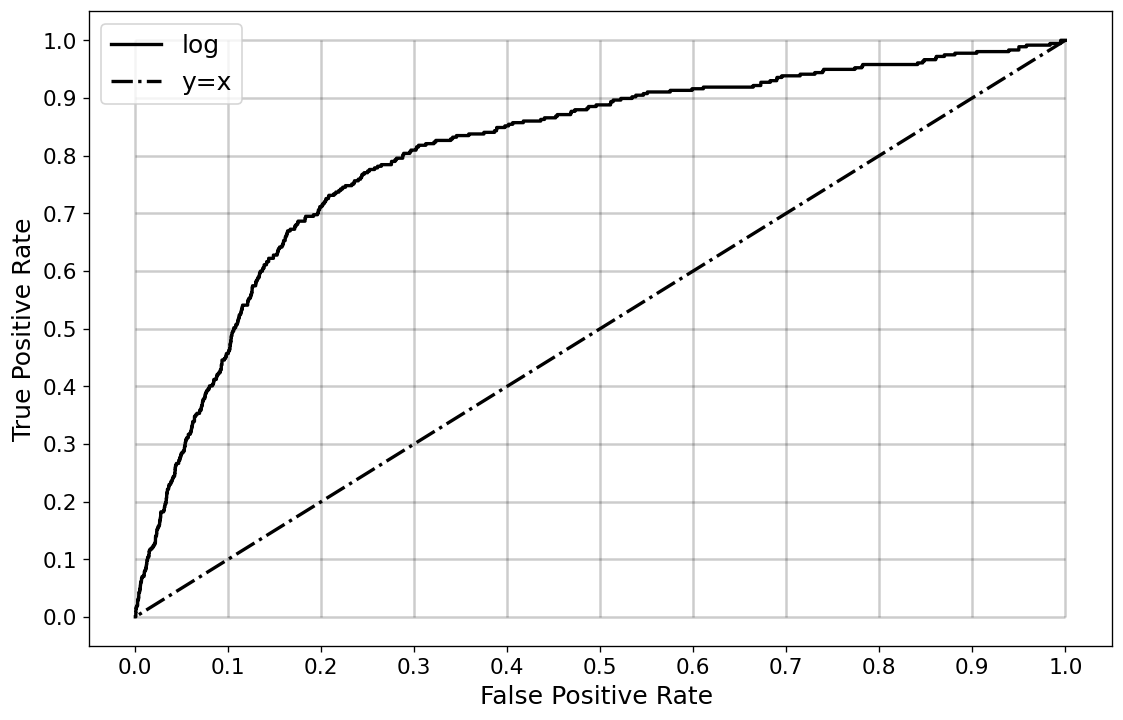
\includegraphics[width=\textwidth]{../img/ROC.png}
    \caption[ROC curve]{The ROC curve.}
    \label{fig:ROC}
\end{figure}

\begin{table}[h]
    \centering
    \begin{tabular}{lrrrrrrr}
        \toprule
        FPR (\%) &  5.05 & 10.07 & 15.08 & 20.82 & 30.22 & 63.02 & 80.01 \\
        TPR (\%) & 30.46 & 49.01 & 62.25 & 74.17 & 82.45 & 92.05 & 96.69 \\
        \bottomrule
    \end{tabular}
    \caption{Some specific ($FPR$, $TPR$) points (as percentages) from the ROC curve shown in Figure \ref{fig:ROC}.}
    \label{tbl:ROCpoints}
\end{table}

In order to make the results of this study comparable to another homelessness prediction study, the results of each model evaluated using K-Folds, $k=4$, when the $TPR$ is near 92\% are listed in Table \ref{tbl:perfAtRec092}. These results represent the single point on the ROC curve at ($FPR$, $TPR$) = (0.6302, 0.9205) in Figure \ref{fig:ROC}. 

\begin{table}
    \centering
    \begin{tabular}{lcccccc}
        \toprule
        Class & Actual & Predicted &  Hits &  TPR (TNR) &  Precision &  f-1 \\
        \midrule
        Positive &    302 &     53243 &   278 &       0.92 &       0.01 & 0.01 \\
        Negative &  84043 &     31102 & 31078 &       0.37 &       1.00 & 0.54 \\
        \bottomrule
    \end{tabular}
    \caption[Performance of model when recall is 0.92]{Performances of model using K-Folds ($k=4$) at threshold where $TPR \approx 0.92$.}
    \label{tbl:perfAtRec092}
\end{table}

%------------------- DISCUSSION ---------------------------------
\chapter{Discussion}
\section{Model Usage}
For model use, a specific binning threshold must be chosen with different thresholds yielding different model performance. For HPPs that plan to target a small segment of the population, a high threshold is appropriate so that only a few predictions are binned as positives. High thresholds correspond to the lower left region of the ROC plot where the $TPR$ and the $FPR$ are both low. For HPPs that plan to target large portions of the population, a low threshold, corresponding to the upper right portion of the ROC plot, is appropriate. 

Since the method of K-Folds was employed, $k=4$ models were actually trained and the overall performance is an average of all the models. If similar performance is to be attained, all models must predict the risk of experiencing homelessness for a new person, then the average prediction will be the prediction of the overall method.

\section{Variability of Evaluation}
As mentioned in the Methods Section, model evaluation was highly sensitive to which people were selected for the training set and the test set. The method of K-Folds was employed to mitigate this issue, but evaluation remained variable from run to run because the selection of which people ended up in which fold was random and differed from run to run. This problem is a result of the data imbalance; because the models have so few positive cases to learn from, the makeup of those positive cases is important. If the random split happens to select positive cases for the training set that are different from the test set, then the model will have more difficulty identifying those positive cases in the test set. 

The choice of $k$ also had an effect on model evaluation. Over several runs it was found that the best model performance was achieved from $k=2$ to $k=5$. For balanced datasets, performance is generally increased with increasing $k$ until about $k=10$ where performance does not increase significantly if $k$ is increased further. Training on large datasets, at least 5000 entities, can achieve good results with $k$ values as low as 5. Typically $k=10$ is used by convention \cite{marcot2020optimal}. With imbalanced data, however, if the value of $k$ is large then there are very few positive cases in the test set, so the models have difficulty distinguishing this small set from all the negative cases. This is likely the reason why lower $k$ values were found to produce better performance for this study.

\section{Model Performance}
The performance of the model is relatively low, but should be interpreted with two considerations. The first consideration is the incompleteness of the data. Before any models are run, of all the people in the data labeled as positive, our confidence that they are actually positive is high - they matched someone who was recorded as experiencing homelessness in the Spokane area. Our confidence in the correct labeling of the negative cases, on the other hand, is lower. Some of the cases labeled as negative in the data may, in reality, be positive cases if they did experience homelessness but this was not recorded in the City of Spokane CMIS database. Because some of the negative cases may be positive cases in reality, the model may have predicted them as positive because they have similar characteristics to other positive cases, but that prediction was labelled as incorrect. This is an unknown factor in this data, but it may cause the model performance to appear worse than it actually is.

Another point of interest is that the people predicted as positive by the models may be members of a more general at-risk population. The only outcomes we measured were related to homelessness, but the model predictions and the data investigation reveal that many people labeled as negatives have similar characteristics to the positive cases. These $F_P$'s may be financially stressed or at-risk in other ways, but we did not have data on other types of outcomes to investigate this.

The other aspect to consider when interpreting model evaluation is the performance of current methods of homelessness prediction. The performances of our models seems low, but perhaps they may be higher than existing methods. In many areas there is no system for predicting homelessness, and, in others where prediction systems do exist, their performance may have never been evaluated.

The only other homelessness prediction paper we found that listed prediction results was from Dr. Beth Shinn's study, \textit{Efficient Targeting of Homelessness Prevention Services for Families} \cite{shinn2013efficient}. This study was conducted on a subgroup of the population in New York that applied for housing assistance and had incomes below 200\% of the national poverty level, instead of the entire population as in our study. Shinn's study tested the Cox Proportion Hazards model, similar in this context to the Logistic Model, and a screening model based on a points system for the purpose of predicting shelter entry on this subpopulation. These models performed similarly, with the screening model achieving a $TPR$ of 91.9\% with a $FPR$ of 65.7\% at the same threshold \cite{shinn2013efficient}. Though this study cannot be directly compared to ours due to the differences in groups upon which predictions were made, the log model in our study achieved similar performance metrics. Listed in Table \ref{tbl:perfAtRec092}, our model achieved a $TPR$ of 92.0\% with a $FPR$ of 63.0\% - just slightly lower performance as compared to Shinn's model. For Shinn's study, a $FPR$ of 65.7\% may be acceptable because the number of false positives is likely small compared to the overall population of New York City, meaning this prediction method is likely efficient when viewed from the population scale. 

\section{Dependence on Time}
It was hypothesized that time is an important factor in predicting homelessness. As people get closer in time to experiencing homelessness they are likely to be more distinguishable from the general population. The history in time of a person's characteristics may be an important factor in predicting homelessness. Two approaches were considered to incorporate individual's previous characteristics in predicting the likelihood of homelessness.

The first approach was to generate naive trajectories for each person over time. This was done by fitting a linear line for each variable in time, then only retaining the slope of the line. This method records the long-term trend of a person in each variable over time. These trends were used as predictors instead of the actual variable values. The performance of the models using these trajectories was lower than the methods discussed so far.

Another method investigated for including a person's previous values as predictors was to take the first difference in each variable of the last two months available for each person. These variable differences capture the local changes in people's characteristics. The differences were used as predictors in the place of the original variable values. Again, model performance was lower here than for the main methods described for this project.

The highest performing method found was to treat each person-place-month combination as a separate entity, make a prediction for each entity, then take the maximum risk prediction for each person over all places and months that person appears in the dataset. This seems to indicate the important aspect of each person is their peak risk. Furthermore, because the outcomes of WITHIN\_6\_MO, and LAST\_MO were less correlated with the predictors than CMIS\_MATCH, an individual's peak risk must not occur immediately before losing their utility account or being evicted. 

\section{Limitations of the Data}
The data used for this project had some limitations that required assumptions to be made. The utility billing data was structured to track accounts and ensure the people responsible for those accounts paid their bills on time. The utility company is a private organization and interested in tracking who is paying for each account so this data structure is appropriate for their uses, but it was not convenient for predicting homelessness.

There were often multiple people associated with a single utility account. These were likely people like spouses, parents, cotenants, or landlords. With these multi-person accounts, it was not recorded who, out of the people associated with the account, paid for each bill. For this project it was assumed that the main account holder always paid since they were ultimately financially responsible for the account, but this is likely not always true. There may be useful information regarding who paid a utility bill for each month; specifically, it may be a risk indicator if someone other than the main account holder paid the bill for a given month.

Another limitation to the billing data was that Avista and City utility billing information was matched using address, not person, so it is unknown if the same person actually paid both bills. This choice was made because matching on address and month across the billing systems of Avista and the City of Spokane had a much higher match rate than matching on the recorded account holder names. It is likely that many of the City utility bills for apartments were paid by the landlord and so would remain unaltered if the tenant was experiencing financial stress. This aspect is addressed, to some degree, by the selection of explanatory variables. It was found that the aggregated measure TOTAL\_60\_DAYS\_AMT, the combined amount owed to Avista and the City for bills over 60 days old, was most associated with the outcome measure out of all other variables related to amount owed. This indicates that even if many landlords did pay consistently for the City utilities even for people who were at risk of homelessness, there was enough information in the amounts owed in City utilities regarding homelessness that aggregating the Avista and City amounts owed produced a variable more strongly associated with CMIS\_MATCH than the individual variables.

Another limitation, as mentioned previously, is that the data on the outcome measures are likely incomplete. If people move away or never report their status of homelessness, they are not captured by the CMIS database and are not labeled as a positive case. This is likely a problem with predicting homelessness, to some degree, on any scale and in any location - even if there were a national homelessness tracking system some people would still move out of the country or not report their homelessness status.

Location was hypothesized to be an important predictor of homelessness, but there were challenges with including location as a predictor in the models. The variables available that contain geographical location information were POSTAL, the person's postal code, BLOCKGROUP\_GEOID, the U.S. Census blockgroup number, and SPA\_PREM\_ID, the assigned identification number for a specific residence. The unit of blockgroup is smaller than that of postal code, but blockgroup areas often do not fall within a single postal code boundary. All of these variables are categorical with POSTAL having 17 unique levels represented in the data, BLOCKGROUP\_GEOID having 279, and SPA\_PREM\_ID having 60785. Because these categorical variables had so many possible values, they could not be incorporated into the logistic model without causing convergence issues.

%------------------- BIBLIOGRAPHY ---------------------------------
\bibliography{CM_Thesis_Pub_Bibliography}
\bibliographystyle{plain}

\end{document}
